\begin{figure}[H]
    \begin{subfigure}[t]{0.33\textwidth}
        \caption{}
        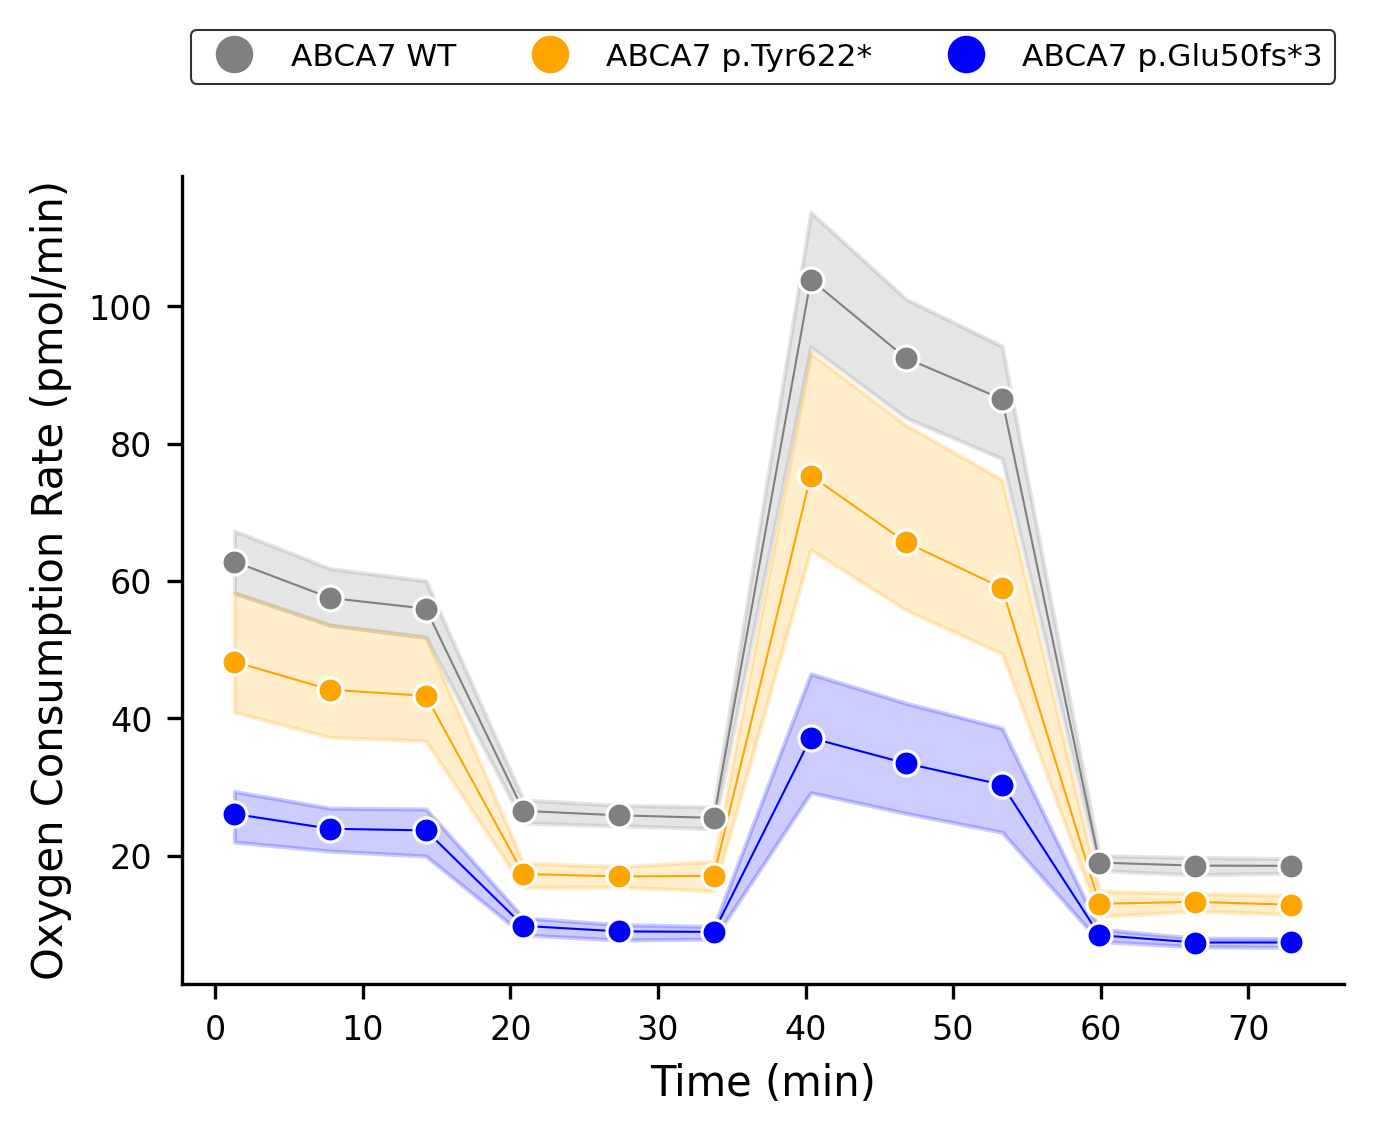
\includegraphics[width=\textwidth]{../paper/extended_plots/rep_seahorse_curves_by_line.png}        
    \end{subfigure}
    \begin{subfigure}[t]{0.33\textwidth}
        \caption{}
        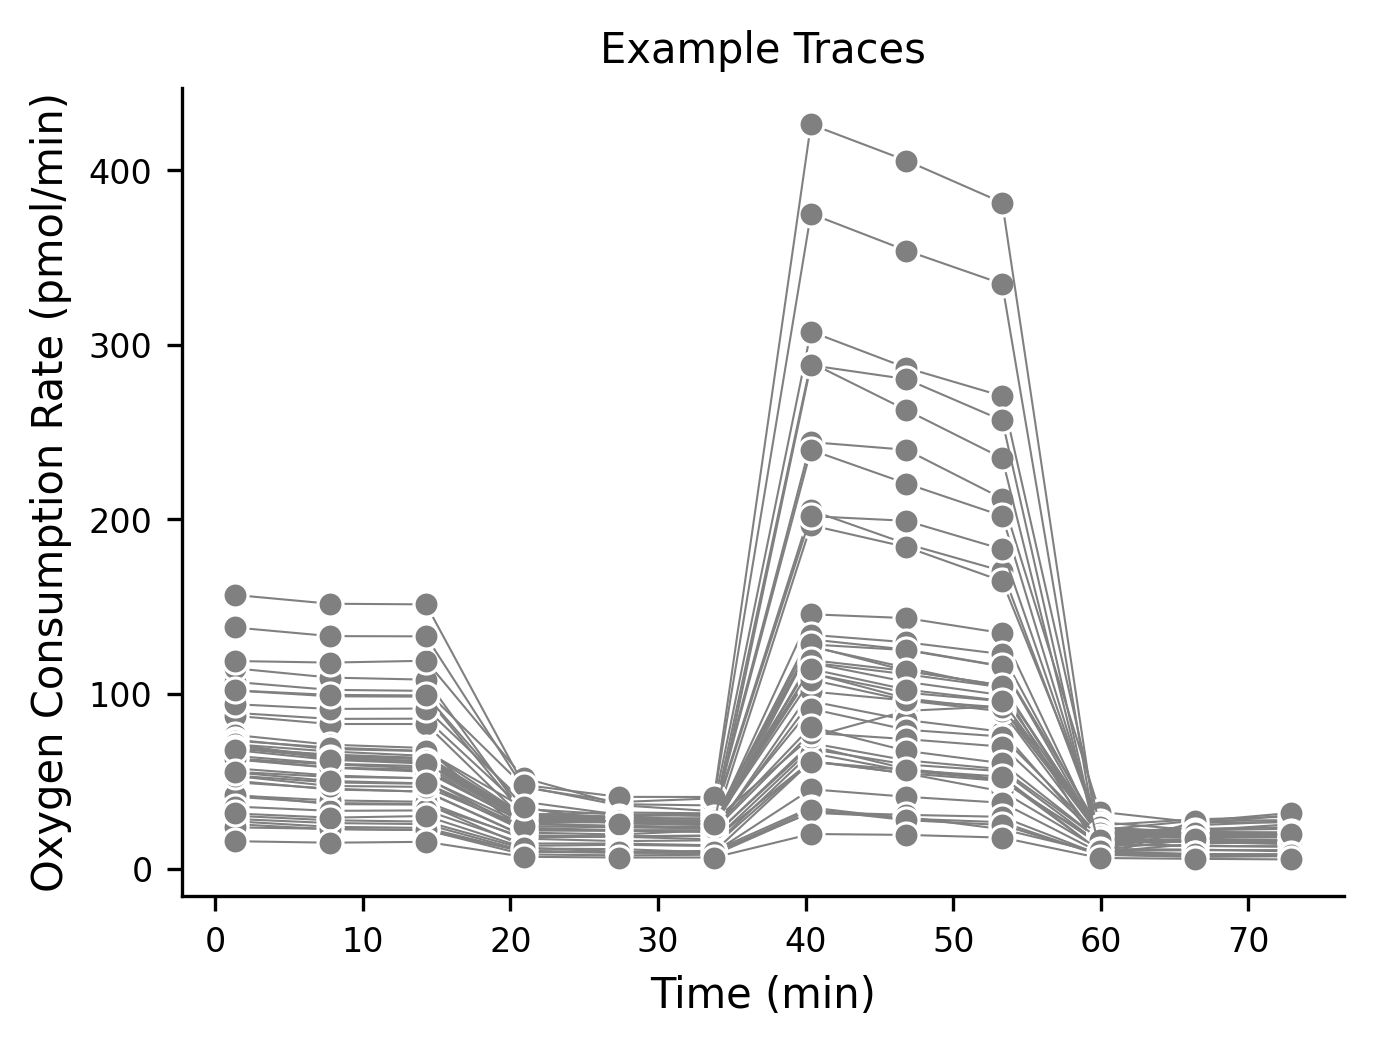
\includegraphics[width=\textwidth]{../paper/extended_plots/rep_seahorse_curves_all.png}        
    \end{subfigure}   
    \begin{subfigure}[t]{0.33\textwidth}
        \caption{}
        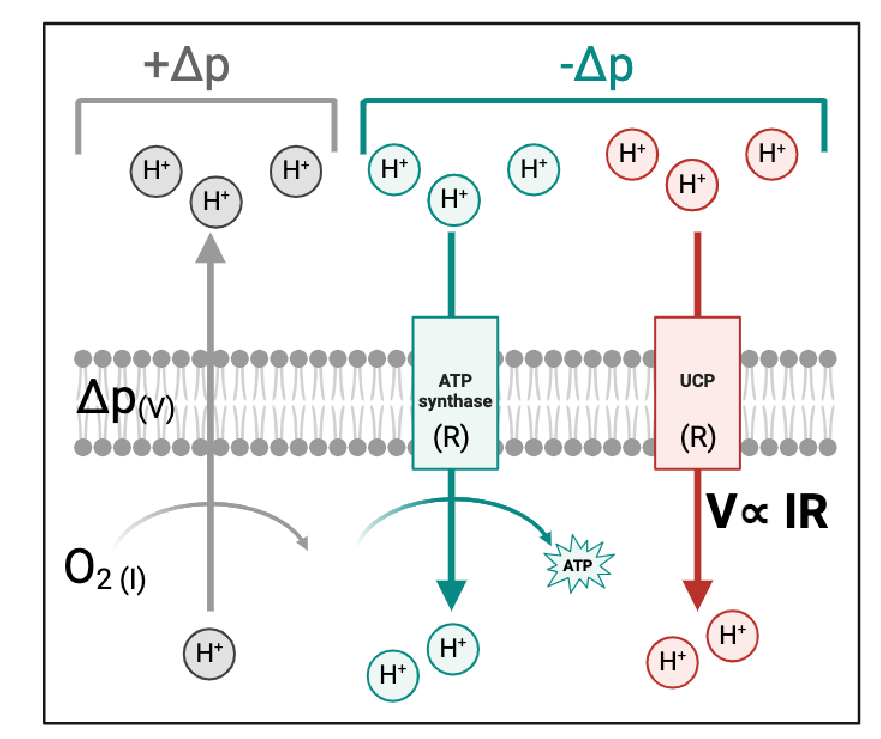
\includegraphics[width=\textwidth]{../paper/main_plots/uncoupling_cartoon.png}        
    \end{subfigure}  
    \begin{subfigure}[t]{0.33\textwidth}
        \caption{}
        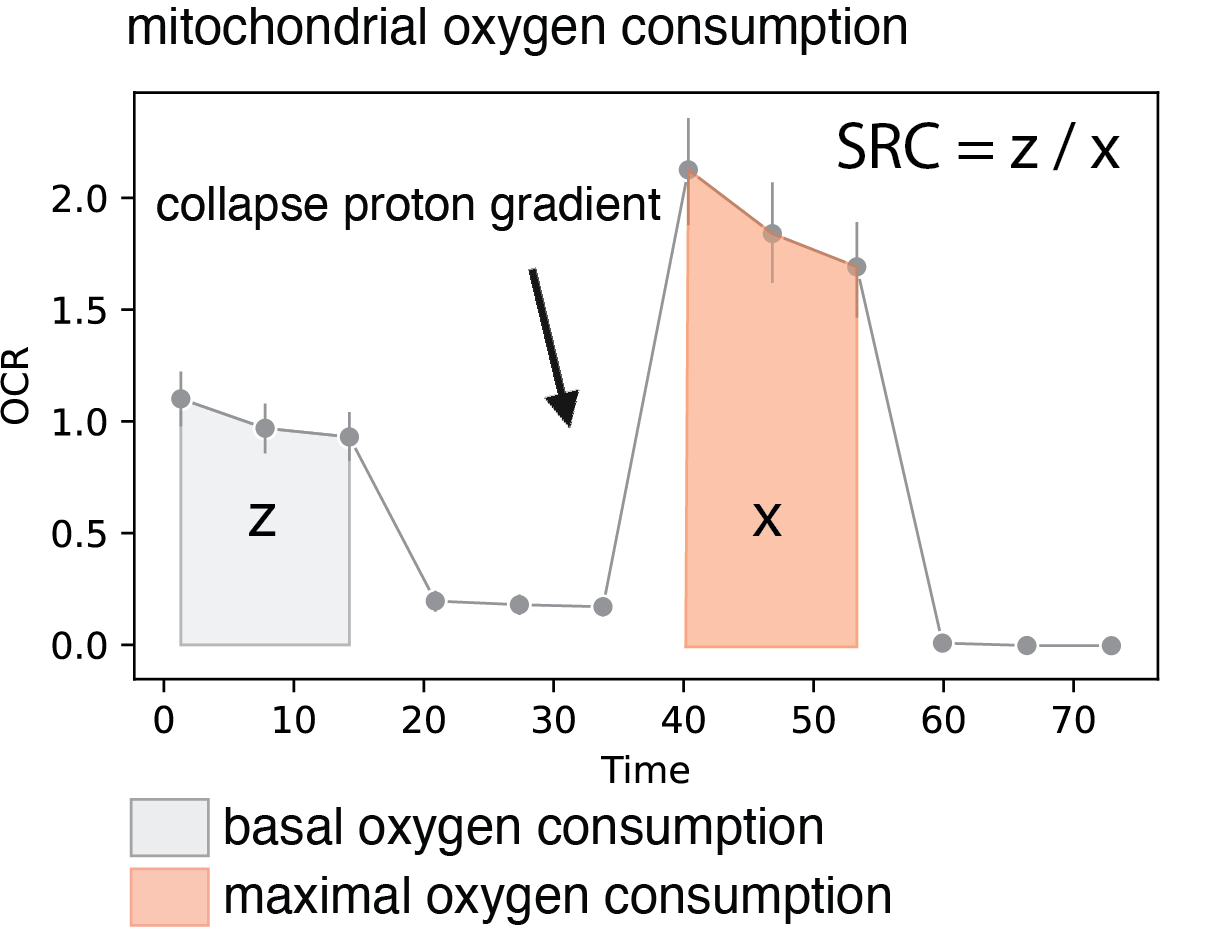
\includegraphics[width=\textwidth]{../paper/extended_plots/src_cartoon.png}        
    \end{subfigure} 
    \begin{subfigure}[t]{0.25\textwidth}
        \caption{}
        \includegraphics[width=\textwidth]{../paper/extended_plots/SRC.png}        
    \end{subfigure} 
    \begin{subfigure}[t]{0.33\textwidth}
        \caption{}
        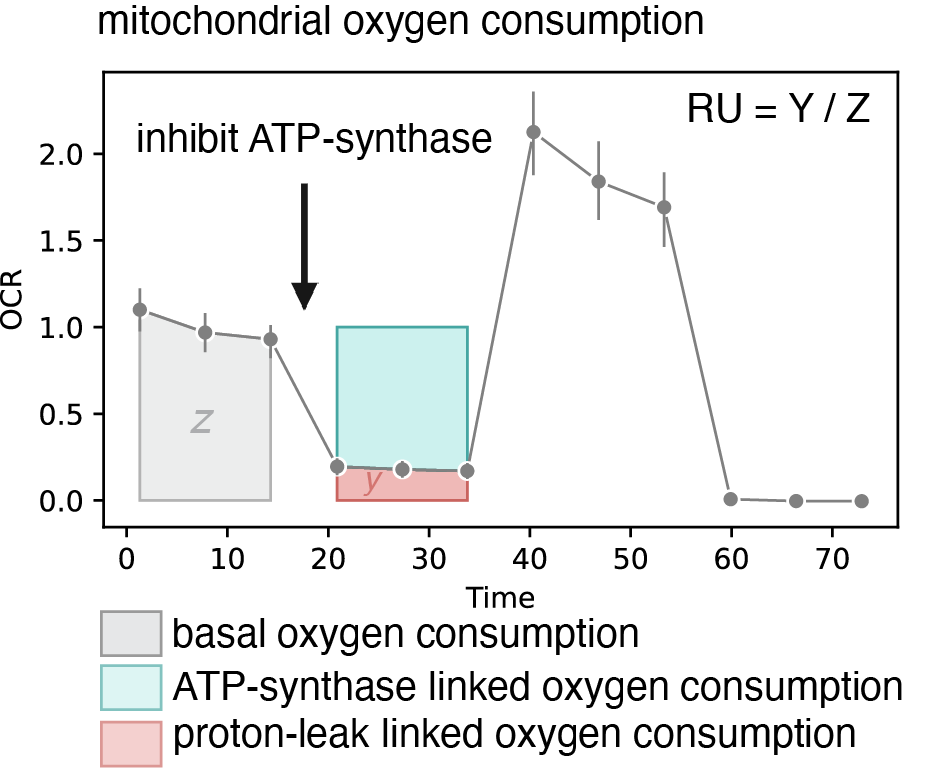
\includegraphics[width=\textwidth]{../paper/main_plots/seahorse_cartoon.png}        
    \end{subfigure}  
    \hspace{1cm}
    \begin{subfigure}[t]{0.3\textwidth}
        \caption{}
        \includegraphics[width=\textwidth]{../paper/extended_plots/UCP_levels.png}        
    \end{subfigure} 
    \par
    \centering
    \begin{subfigure}[t]{0.65\textwidth}
        \caption{}
        \includegraphics[width=\textwidth]{../paper/main_plots/tmrm_with_FCCP.png}        
    \end{subfigure} 
 \end{figure}
\textbf{Extended Data Fig. 10}